\documentclass[5p]{elsarticle}
\usepackage{graphicx}

\begin{document}
\begin{frontmatter}
\title{An overview of the Data for Jooriland\tnoteref{t1}}
\tnotetext[t1]{This document is designed to provide a quick overview of the data.}
\author[jsl]{Jason Lessels}
\address[jsl]{The University of Sydney}
\ead{j.lessels@usyd.edu.au}
\begin{abstract}
This article is designed to provide an overview of the data being used to optimise the sampling scheme currently used by the SCA. Current
\end{abstract}
\begin{keyword}
\end{keyword}

\end{frontmatter}
\section*{Introduction}
Water quality sampling is common place and required by law to allow catchment management agencies to maintain the health of a catchment. It is now well established that Australian streams have the highest levels of nutrient exports during storm events. Due to this relationship, sampling schemes are currently shifting from a monthly sampling basis, to a event-based sampling scheme. The shift has caused a necessary shift in the statistics that are currently used to analyses the data.

The data obtained from the Sydney Catchment Authority (SCA) has a continuous discharge data set starting early 1960 and ending in 2009. The water quality dataset currently being used was supplied mid 2008. This dataset starts in 1991 and ends in 2008. This dataset is heavily biased with the starting of this dataset, being only collected via routine and flood, samples. This bias leads to the belief that the data in the early part of the data set has missed several key events.
\section*{Background}
The Sydney Catchment Authority is in charge of the drinking water for the metropolitan area of Sydney. The catchment is a large catchment, that stretches from Gouldburn in the South to Bathurst in the North. The catchment is characterized by low lying hills in the south, which is dryer th...

\section*{Data Summary}
The data collected from the SCA covers a variety of variables. This paper will only cover EC,TP,TN,and NTU variables. An overview of the data is provided in table \ref{table:summary_stats}. Correlation plots between the variables are also provided in figure \ref{fig:correlation_plots}. The correlation plots provide an overview of the relationships between the various water quality variables and the associated discharge. 

% Fri Nov 20 13:04:05 2009
\begin{table}[ht]
\begin{center}
\caption{Summary statistics of data}
\begin{tiny}
\begin{tabular}{rrrrrrr}
  \hline
Statistic & pH & EC & NTU & TN & TP & Discharge \\ 
  \hline
Min & 6.50 & 0.02 & 0.54 & 0.17 & 0.00 & 0.00 \\ 
  Max & 9.16 & 0.71 & 1000.00 & 14.80 & 2.28 & 2507.99 \\ 
  Mean & 7.84 & 0.29 & 67.43 & 0.87 & 0.07 & 163.40 \\ 
  Median & 7.80 & 0.30 & 15.70 & 0.60 & 0.02 & 42.03 \\ 
  Stdev & 0.53 & 0.11 & 140.88 & 1.00 & 0.15 & 335.10 \\ 
  n & 285.00 & 1125.00 & 1314.00 & 523.00 & 513.00 & 1375.00 \\ 
   \hline
\end{tabular}
\end{tiny}
\label{table:summary_stats}
\end{center}
\end{table}
The samples of the water quality variables have been collected using a variety of methods. These methods are summarized in table \ref{table:sample_types}. Figure blah shows the correlation between discharge and total Phosphorus, for each sample type.

\begin{table}[ht]
\begin{center}
\caption{Quanity of sample types in relation to water quality variable}
\begin{tabular}{lrrrrr}
  \hline
 Sample type & pH & EC & TP & TN & NTU \\ 
  \hline
  unknown &  60 &   0 & 128 & 128 & 120 \\ 
  automatic &  25 & 850 & 121 & 124 & 926 \\ 
  composite &   1 &  35 &  25 &  31 &  35 \\ 
  duplicate &   3 &   3 &   4 &   4 &   3 \\ 
  flood &   0 &  22 &  19 &  18 &  18 \\ 
  N &   0 &   0 &   0 &   0 &   0 \\ 
  monthly grab & 166 & 167 & 168 & 168 & 165 \\ 
  ad-hoc grab &  30 &  39 &  38 &  40 &  38 \\ 
  W &   0 &   9 &  10 &  10 &   9 \\ 
   \hline
\end{tabular}
\label{table:sample_types}
\end{center}
\end{table}

It is important to examine the effect of the sample type, on the quality of the desired relationship. A brief example of this is shown in figure \ref{fig:sample_scatter}.


\begin{center}
\begin{figure}
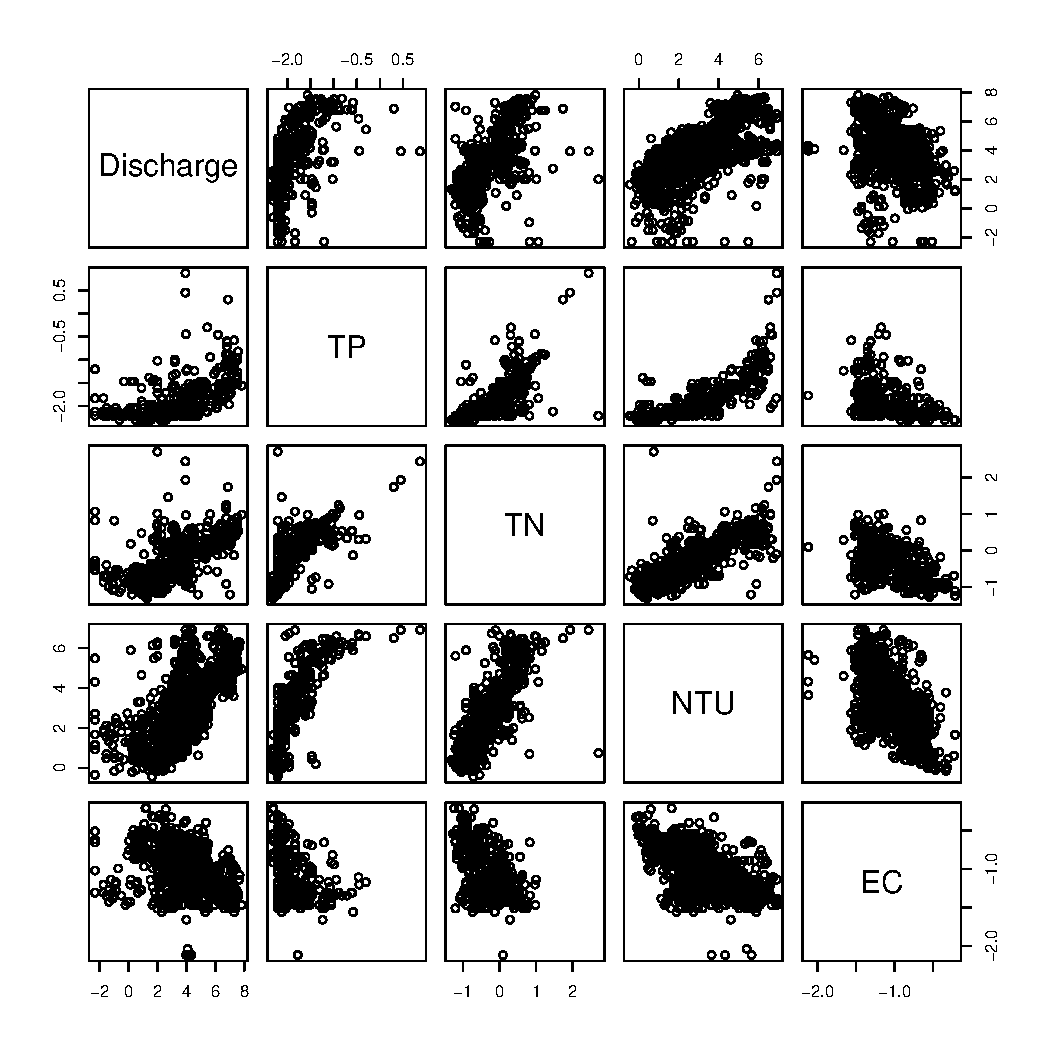
\includegraphics[scale=0.50]{Scatterplotmatrix.pdf}
\caption{Scatter plot of water quality variables.\it{All variables are log transformed.}}
\label{fig:correlation_plots}
\end{figure}
\end{center}

\begin{center}
\begin{figure}
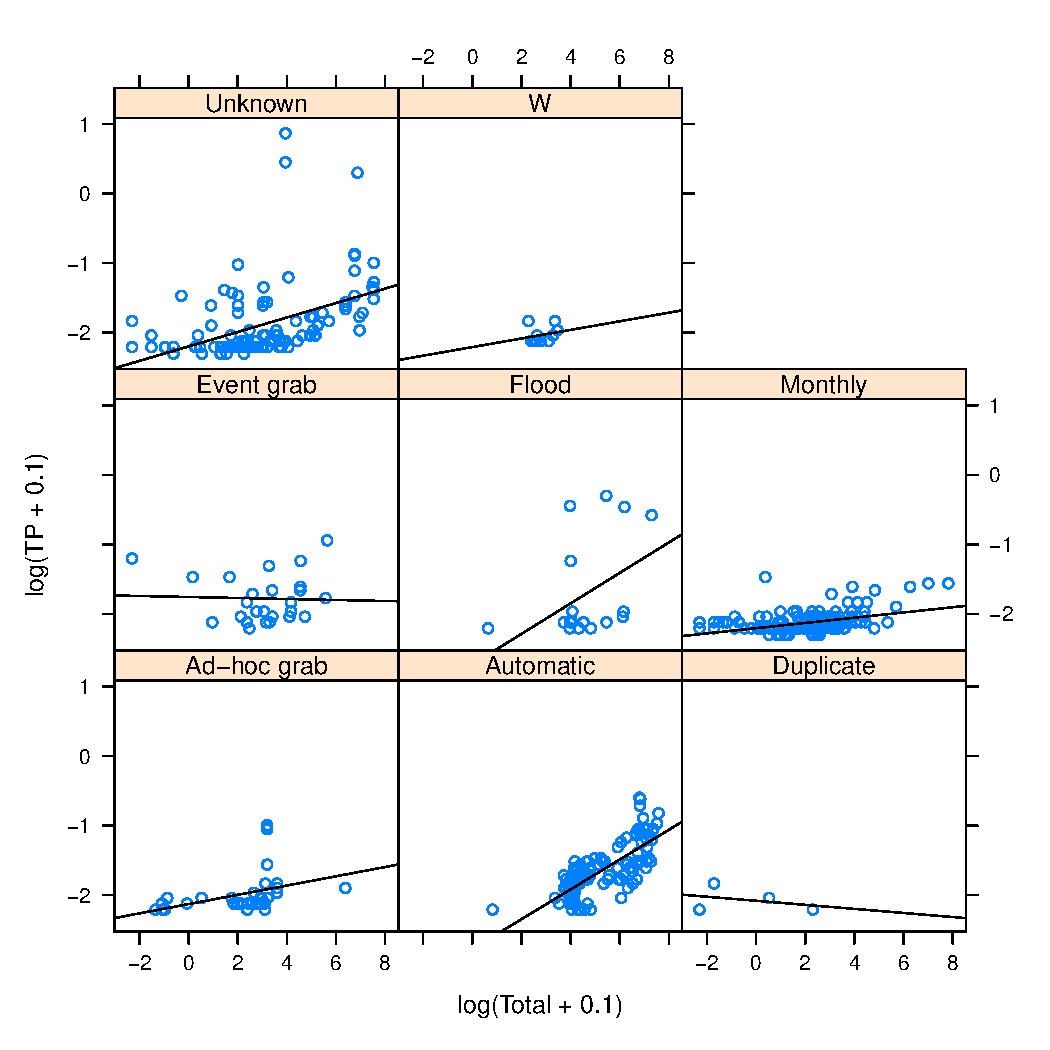
\includegraphics[scale=0.5]{sample_tp_scatter.pdf}
\caption{Scatter plot of total Phosphorous and discharge relevant to each sample type. \it{All variables are log transformed.}}
\label{fig:sample_scatter}
\end{figure}
\end{center}


\subsection*{Transformation of data}
Data related to stream flow in Australia is often highly skewed, due to the nature of the system. It is therefore necessary to transform the data for regression based analysis. The most common technique is the use of the natural log transformation. Various methods are now possible to be used to transform the data. This report will use the flexibility of the box-cox transformation, which can if appropriate use the natural log transformation. The distribution of most of all variables is shown in figure \ref{fig:histograms}.\\
Figure \ref{fig:lambda_example} shows the range of possible lambda values for the transformation of total Phosphorous, with 95\% confidence intervals.\\
Figure \ref{fig:transformations} represents two different transformations of total Phosphorous and discharge. The two types of transformations are the natural log, and the box cox transformation. These transformations required positive data, both the TP and the discharge required an additiion of 0.01 to each observation. To perform the the box cox transformation, the geoR and the TeachingDemos packages where used within R. 



\begin{center}
\begin{figure}[h]
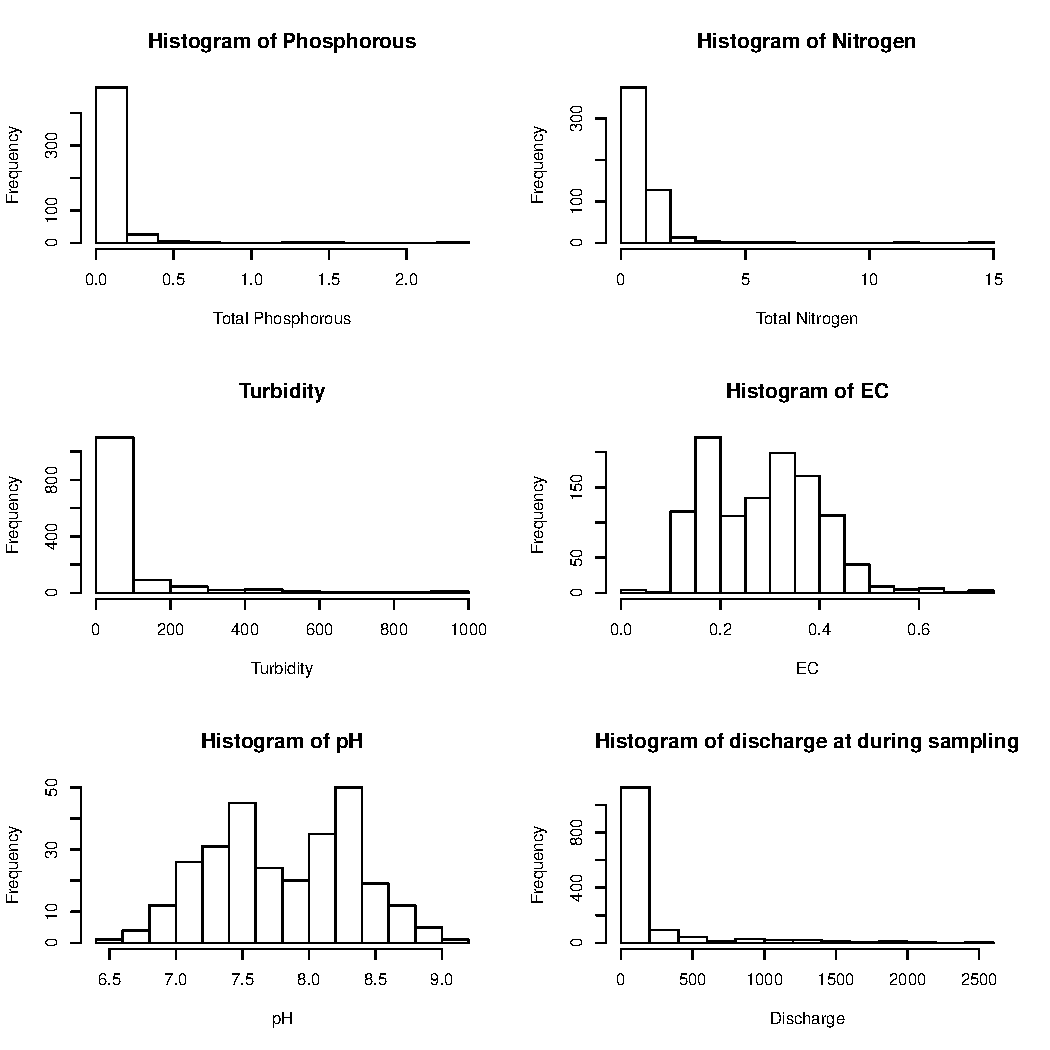
\includegraphics[scale=0.5]{histograms.pdf}
\caption{Histogram of each water quality variable and the associated discharge.}
\label{fig:histograms}
\end{figure}
\end{center}

\begin{center}
\begin{figure}
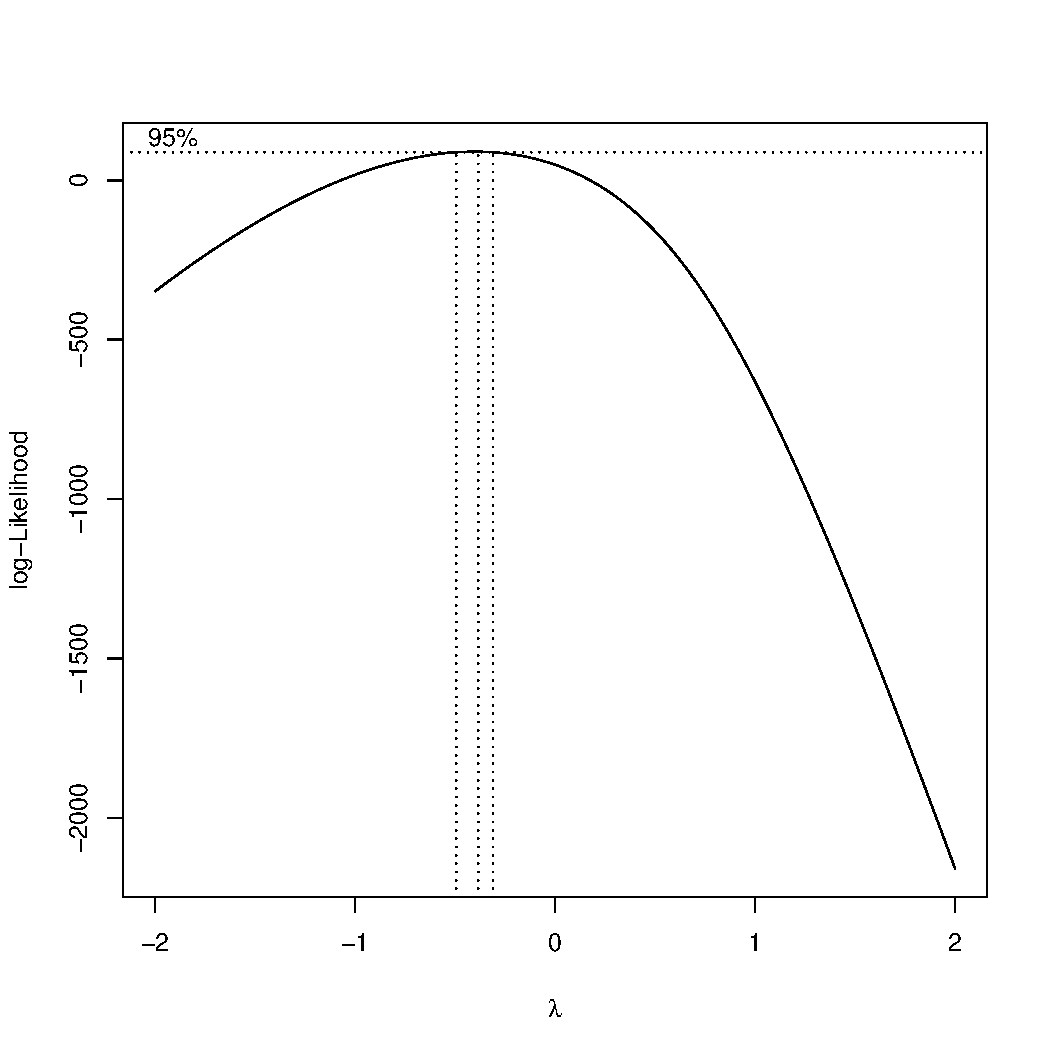
\includegraphics[scale=0.45]{bc_example_tp.pdf}
\caption{Fitted lambda value for the box-cox transformation of total Phosphorous.}
\label{fig:lambda_example}
\end{figure}
\end{center}

\begin{center}
\begin{figure}
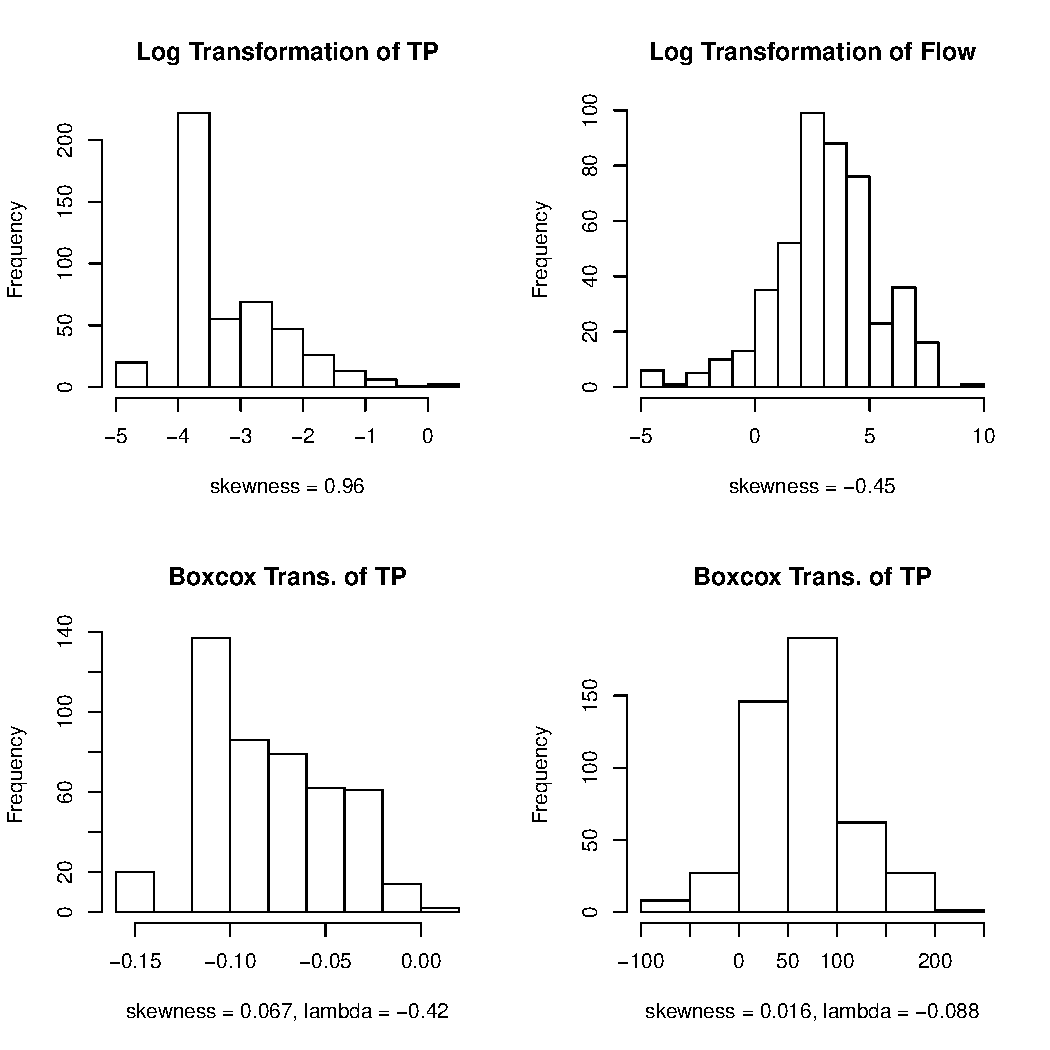
\includegraphics[scale=0.45]{tp_flow_trans.pdf}
\caption{Transformations of total Phosphorous and discharge using log and optimised boxcox transformation.}
\label{fig:transformations}
\end{figure}
\end{center}

\section*{Autocorrelation within the data}
As the data is part of a time series it can be assumed that there is autocorrelation between the samples through time. This section of the report will examine the autocorrelation within the data. It is possible to investigate the discharge data using transnational time series methods. Spatial semi-variograms will be used to examine the autocorrelation with the water quality variables, and the discharge at the associated with the quality samples. Figure \ref{fig:acf_pacf} shows that there is correlation for up to two hours, and the acf shows that that there is a steady rate of decay of correlation. 

\section*{Autocorrelation examination using spatial techniques}
As stated earlier the data is temporal, and therefore it is correlated through time, as shown within \ref{fig:acf_pacf}. Due to the nature of the quality samples being unevenly sampled through time, it is not possible to use the traditional time series analysis techniques. This section will outline the process of using the gstat and geoR packages in R to determine LMCR of the data. This section will only focus on the relationship between discharge and total phosphorous, but will use both transformations examined in \ref{fig:transformations}.


To obtain covari


From using the R package geoR the use of the function likfit was used with the summary of the model given in figure \ref{fig:R_code}.

\begin{center}
\begin{figure}
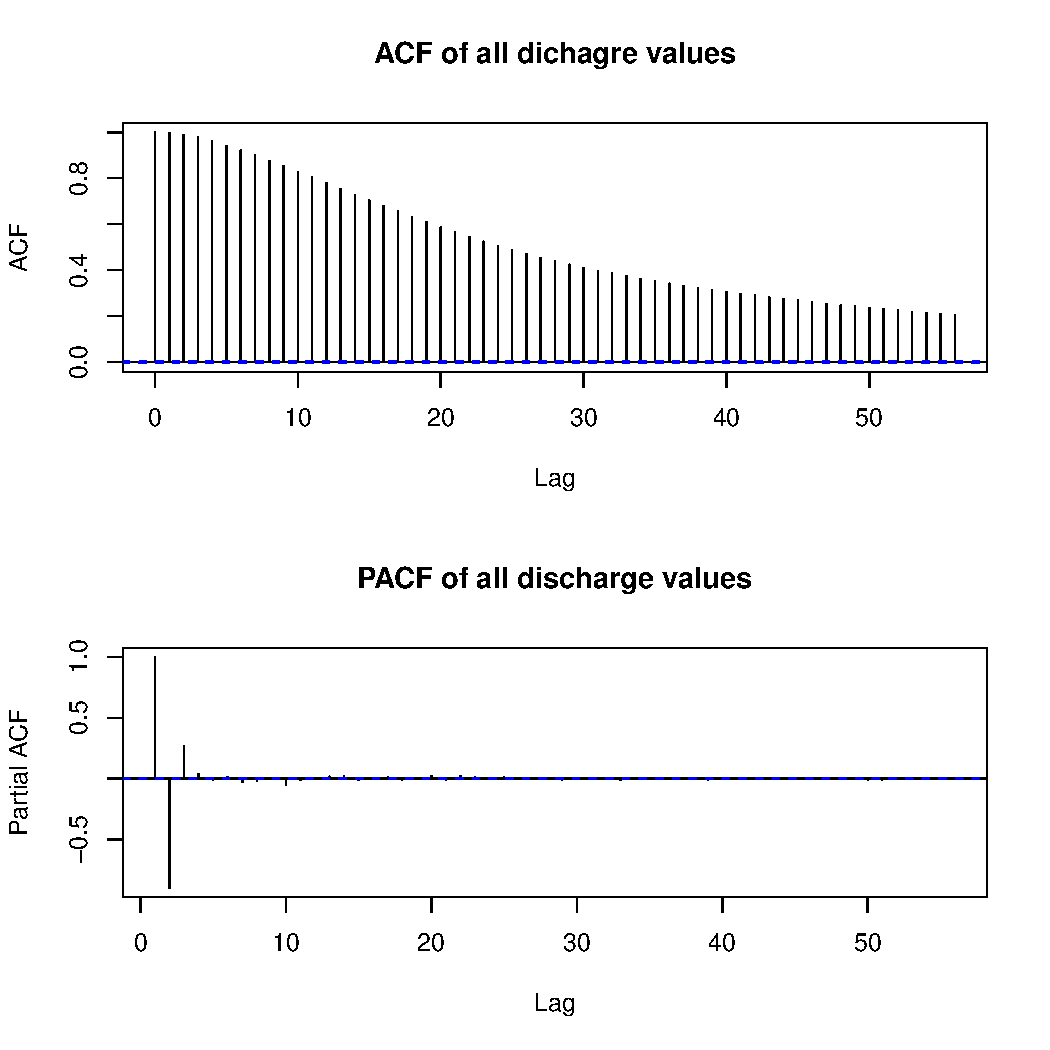
\includegraphics[scale=0.5]{acf_pacf.pdf}
\caption{ACF and PACF of entire discharge time series.}
\label{fig:acf_pacf}
\end{figure}
\end{center}

\begin{figure}
\fbox{
\begin{minipage}{9cm}
\begin{verbatim}

> mlik <- likfit(temp,ini=c(0.5,0.5))

> summary(mlik)

Summary of the parameter estimation\\
-----------------------------------\\
Estimation method: maximum likelihood\\
Parameters of the mean component (trend):\\
   beta \\
-0.0888 \\

Parameters of the spatial component:\\
   correlation function: exponential\\
      (estimated) variance parameter sigmasq 
(partial sill) =  6e-04\\
      (estimated) cor. fct. parameter phi 
(range parameter)  =  21.74\\
   anisotropy parameters:\\
      (fixed) anisotropy angle = 0  ( 0 degrees )\\
      (fixed) anisotropy ratio = 1\\

Parameter of the error component:\\
      (estimated) nugget =  2e-04\\

Transformation parameter:\\
      (fixed) Box-Cox parameter =
1 (no transformation)\\

Practical Range with cor=0.05 for \\
asymptotic range: 65.12826\\

Maximised Likelihood:\\
   log.L n.params      AIC      BIC \\
  "1046"      "4"  "-2083"  "-2067" \\

non spatial model:
   log.L n.params      AIC      BIC 
   "909"      "2"  "-1814"  "-1806" 

Call:
likfit(geodata = temp, ini.cov.pars = c(0.5, 0.5))
\end{verbatim}
\end{minipage}
}
\caption{R output of likfit model of boxcox transformed TP}
\label{fig:R_code}
\end{figure}

From the model the semi variogram cloud is shown in figure 




\end{document} 
